\documentclass{beamer}

\usetheme{CambridgeUS}
\usecolortheme{dolphin}

\usepackage{wrapfig}
\usepackage{siunitx}
\usepackage{inconsolata}
\usepackage{amsmath}
\usepackage{bm}
\usepackage{adjustbox}
\usepackage{nicefrac}
\usepackage{graphicx}

\usepackage[backend=bibtex,style=authoryear]{biblatex}
\bibliography{common/references}
\AtBeginBibliography{\scriptsize}

% Tikz
\usepackage{tikz}
\usetikzlibrary{positioning,shapes,arrows,calc,intersections}
\usepackage{pgfplots}
\usepgfplotslibrary{dateplot}
\pgfplotsset{compat=1.8}

\DeclareMathOperator{\spann}{span}

\definecolor{darkblue}{HTML}{00688B}
\definecolor{darkgreen}{HTML}{6E8B3D}
\definecolor{cadet}{HTML}{DAE1FF}
\definecolor{salmon}{HTML}{FFB08A}

\AtBeginSection[]{
  \begin{frame}
  \vfill
  \centering
  \begin{beamercolorbox}[sep=8pt,center,shadow=true,rounded=true]{title}
    \usebeamerfont{title}\insertsectionhead\par%
  \end{beamercolorbox}
  \vfill
  \end{frame}
}

\begin{document}

\title[Reduced Order Models]{
  Adaptive Isogeometric Methods \\ and Reduced Order Modeling
}
\author[T.~Kvamsdal]{
  T.~Kvamsdal\inst{1,2} \and
  E.~H.~van Brummelen\inst{3} \and
  E.~Fonn\inst{2} \and
  K.~Johannessen\inst{2} \and
  A.~M.~Kvarving\inst{2} \and
  A.~Rasheed\inst{2} \and
}
\institute[NTNU/SINTEF]{
  \and \inst{1}%
  Department of Mathematical Sciences, NTNU
  \and \inst{2}%
  Applied Mathematics and Cybernetics, SINTEF Digital
  \and \inst{3}%
  Department of Mechanical Engineering, TU/e
}
\date[IGA 2018]{}

\titlegraphic{
  \includegraphics[height=0.05\textheight]{common/ntnu} \hspace{0.1\textheight}
  \includegraphics[height=0.05\textheight]{common/sintef} \hspace{0.1\textheight}
  \includegraphics[height=0.05\textheight]{common/tue}
}

\begin{frame}{Basis functions (v, TH and DC)}
  \begin{center}
    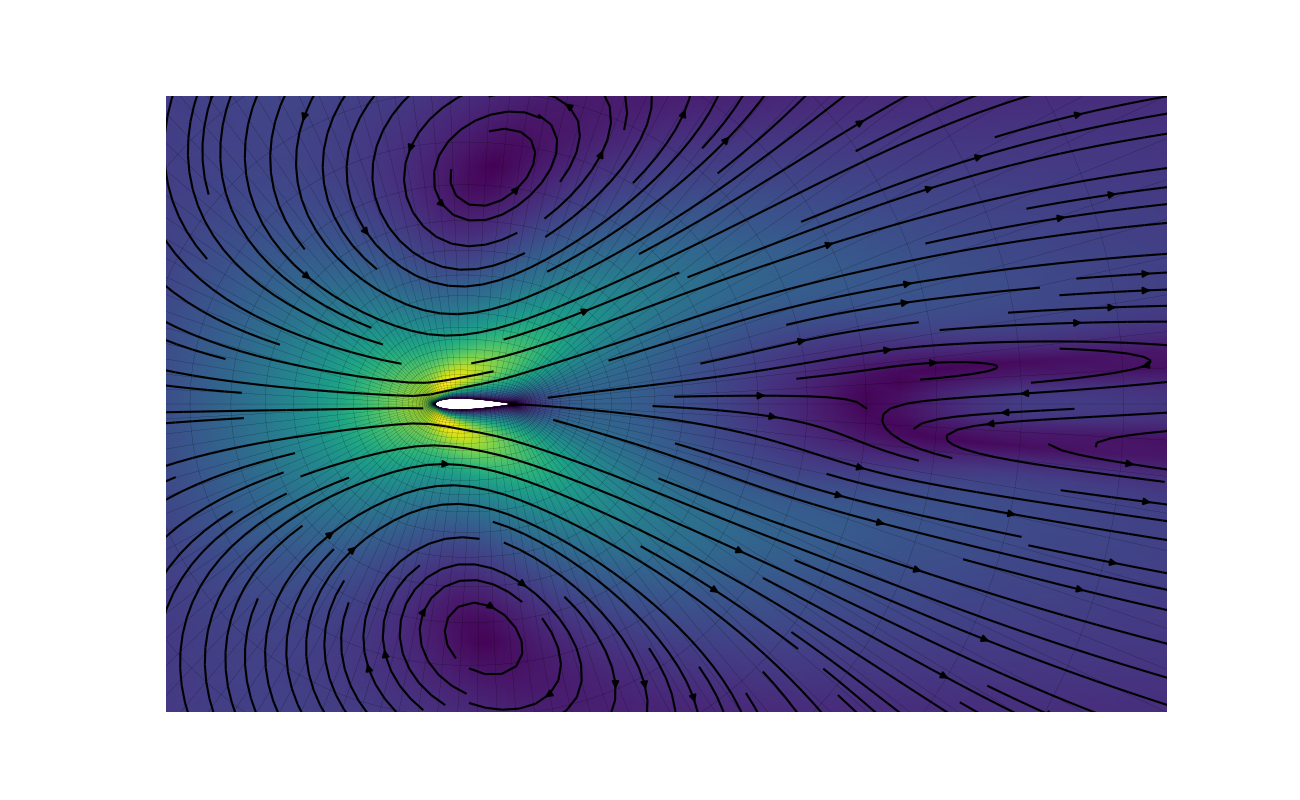
\includegraphics[trim={90mm 0 95mm 0},clip,height=0.95\textheight]{figs/bfun-v-no-piola-v000}
    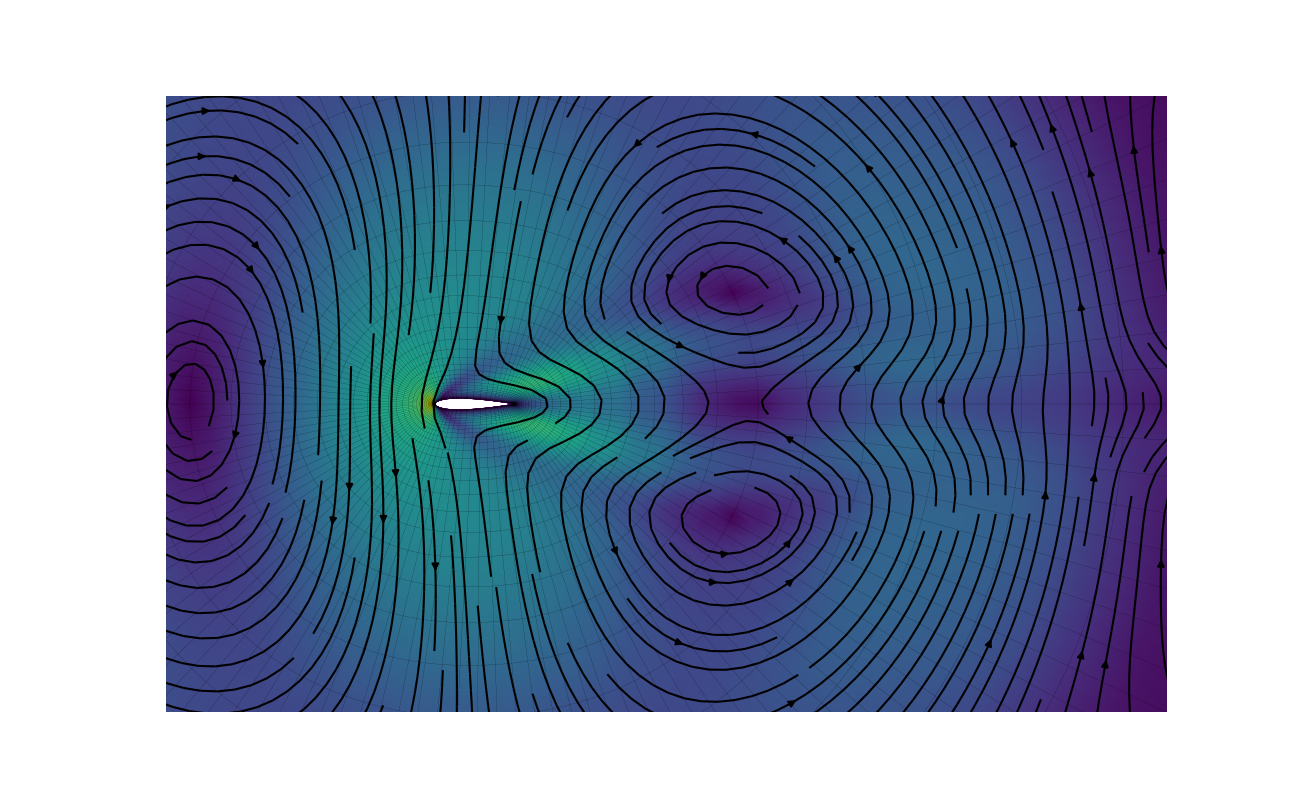
\includegraphics[trim={90mm 0 95mm 0},clip,height=0.95\textheight]{figs/bfun-v-piola-v000}
  \end{center}
\end{frame}

\begin{frame}{Basis functions (v, TH and DC)}
  \begin{center}
    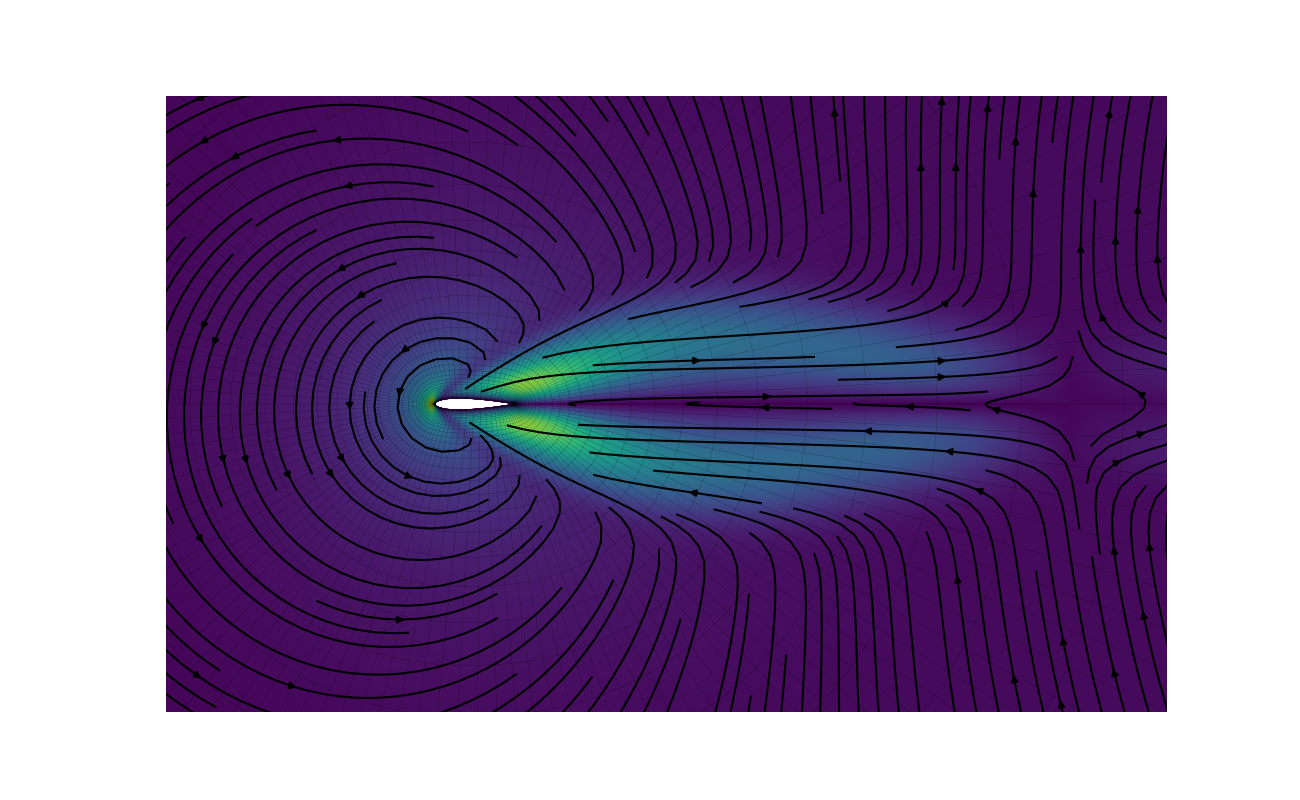
\includegraphics[trim={90mm 0 95mm 0},clip,height=0.95\textheight]{figs/bfun-v-no-piola-v001}
    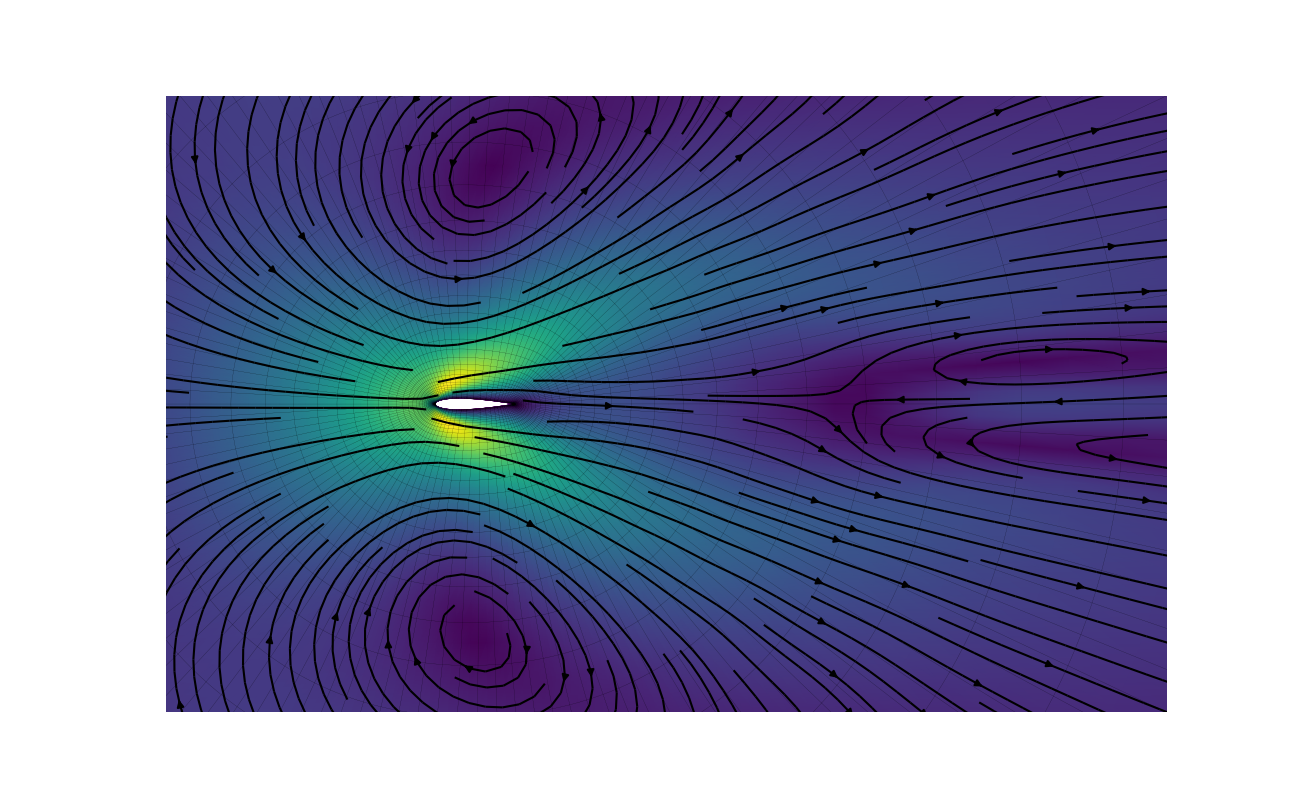
\includegraphics[trim={90mm 0 95mm 0},clip,height=0.95\textheight]{figs/bfun-v-piola-v001}
  \end{center}
\end{frame}

\begin{frame}{Basis functions (v, TH and DC)}
  \begin{center}
    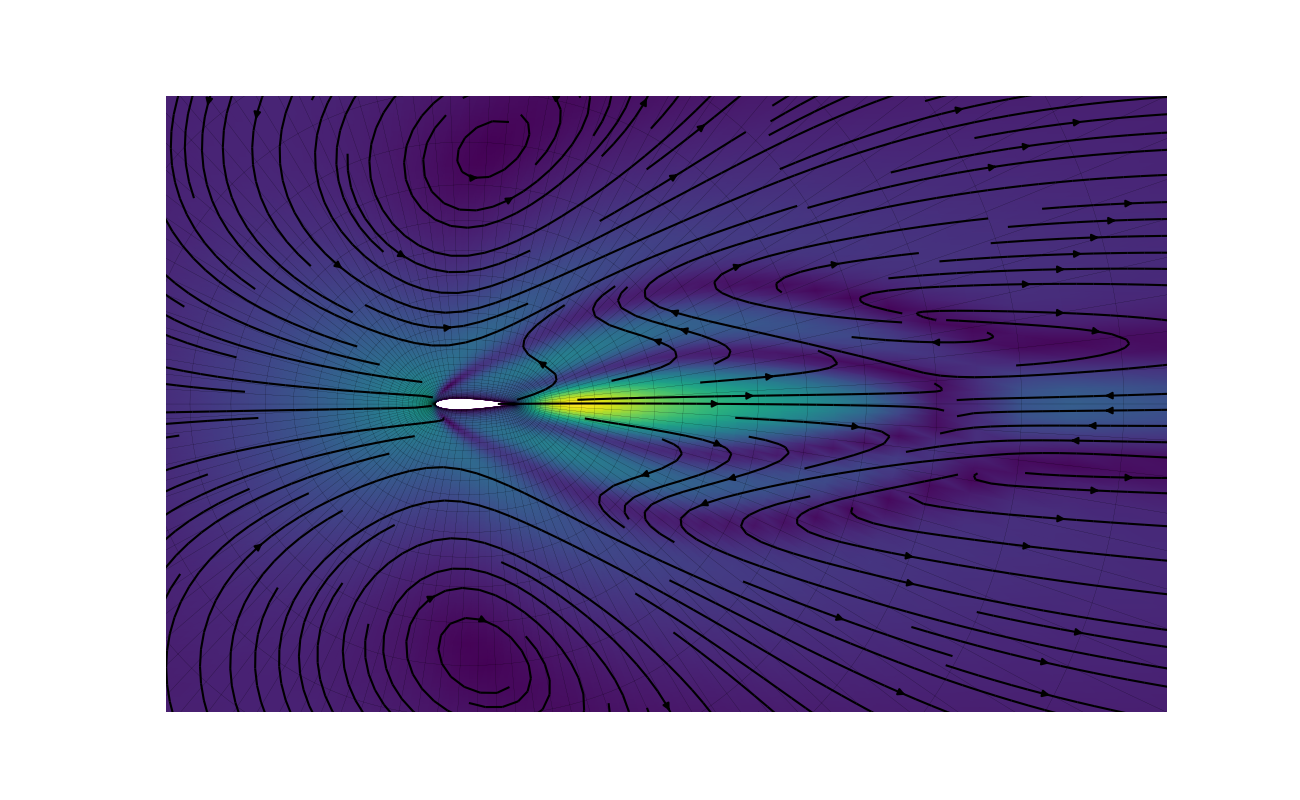
\includegraphics[trim={90mm 0 95mm 0},clip,height=0.95\textheight]{figs/bfun-v-no-piola-v002}
    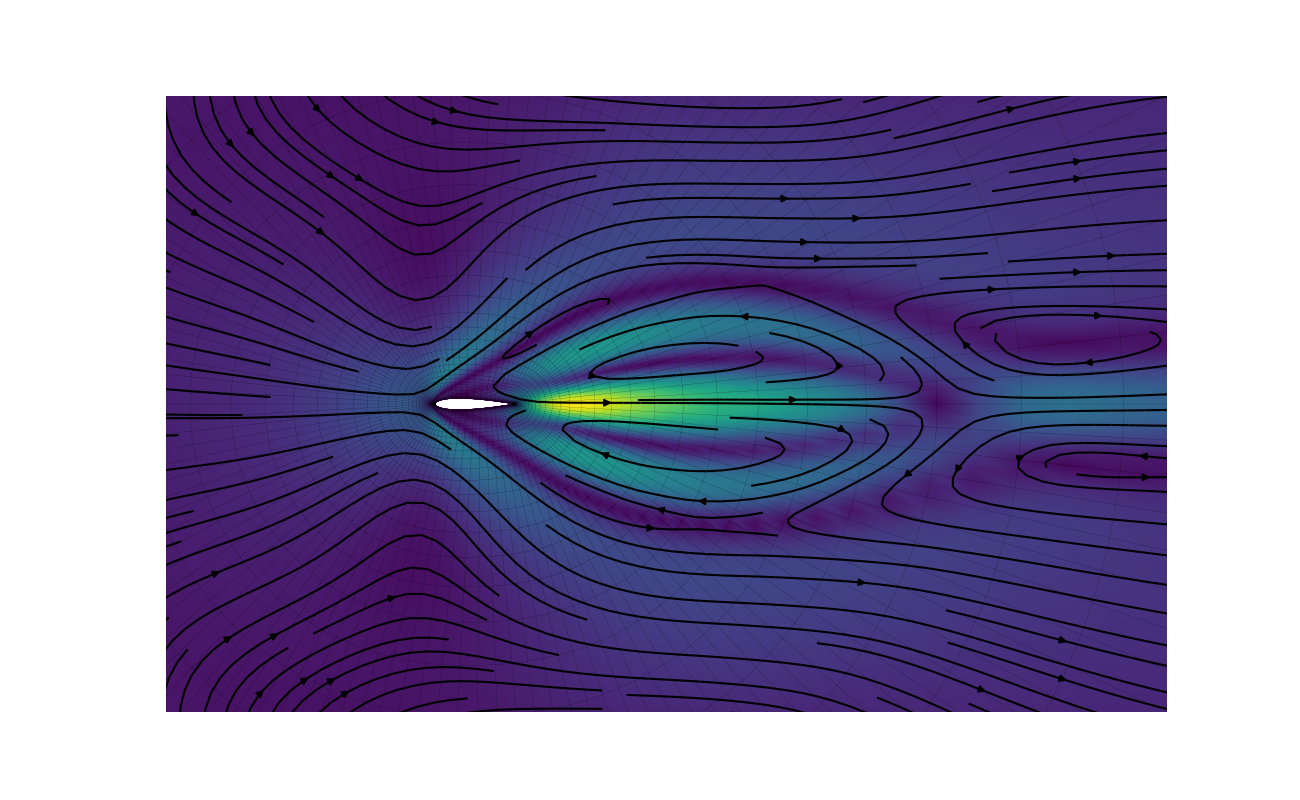
\includegraphics[trim={90mm 0 95mm 0},clip,height=0.95\textheight]{figs/bfun-v-piola-v002}
  \end{center}
\end{frame}

\begin{frame}{Basis functions (v, TH and DC)}
  \begin{center}
    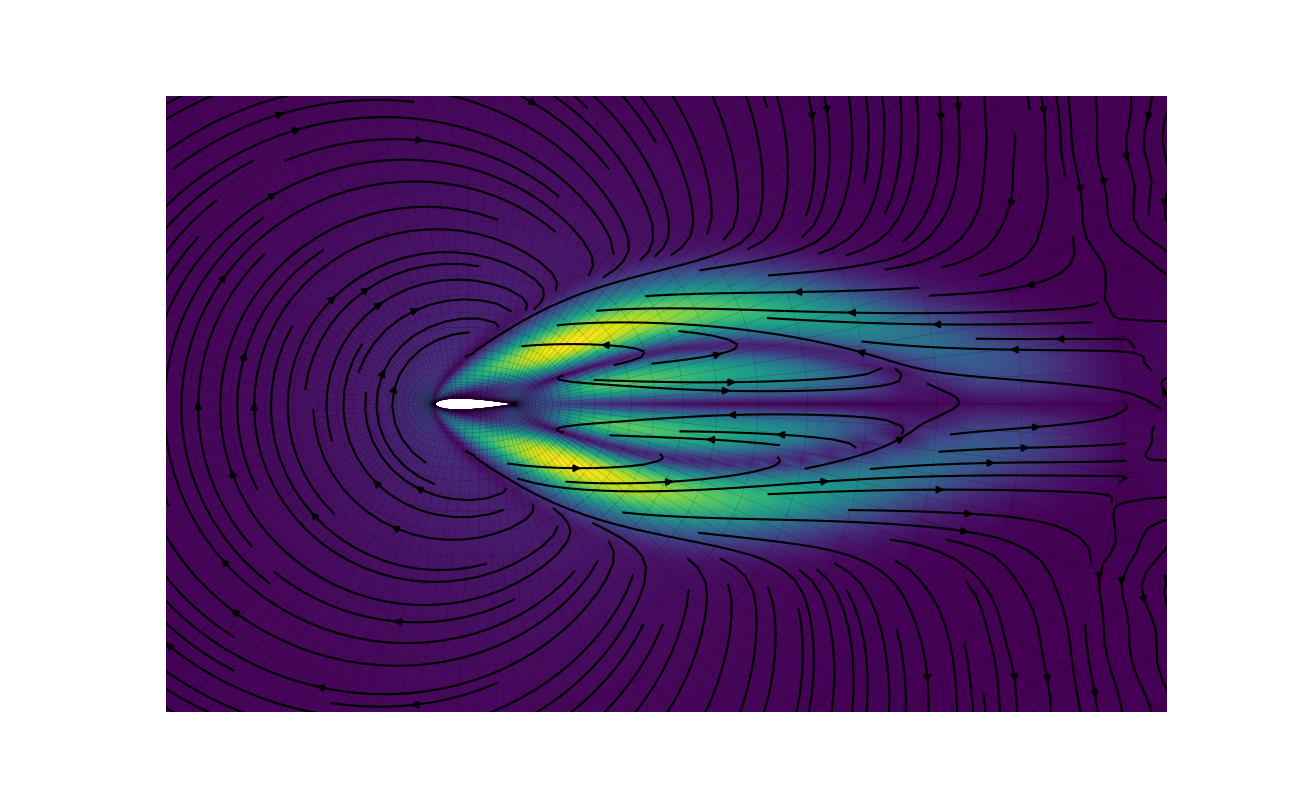
\includegraphics[trim={90mm 0 95mm 0},clip,height=0.95\textheight]{figs/bfun-v-no-piola-v003}
    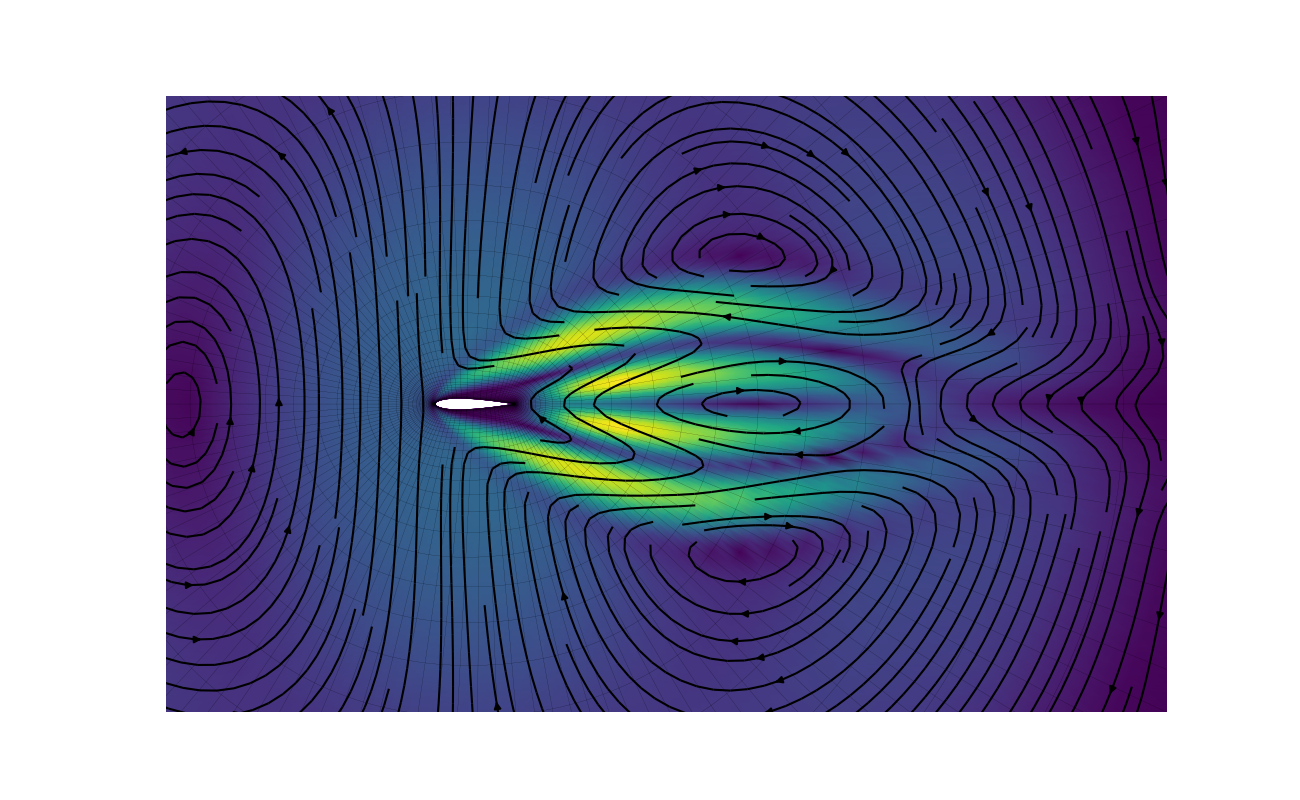
\includegraphics[trim={90mm 0 95mm 0},clip,height=0.95\textheight]{figs/bfun-v-piola-v003}
  \end{center}
\end{frame}

\begin{frame}{Basis functions (p, TH and DC)}
  \begin{center}
    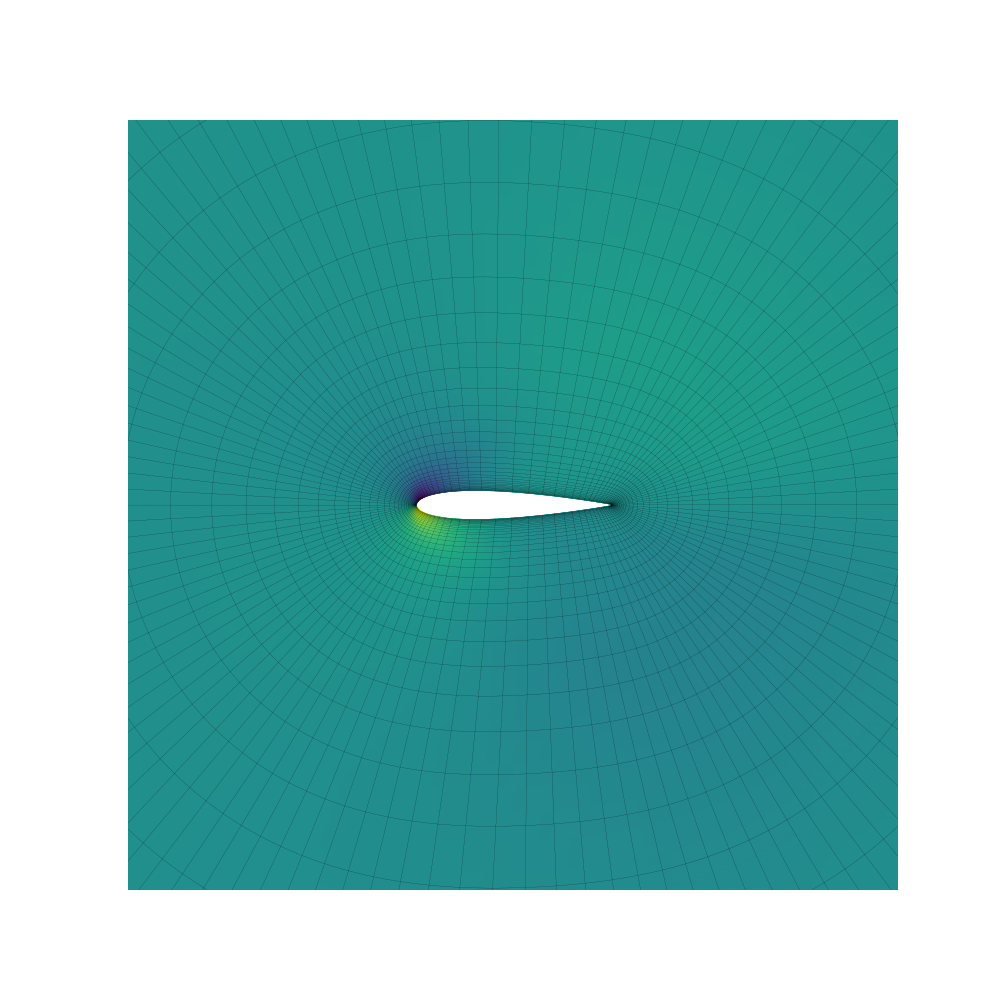
\includegraphics[trim={35mm 0 40mm 0},clip,height=0.95\textheight]{figs/bfun-p-no-piola-p003}
    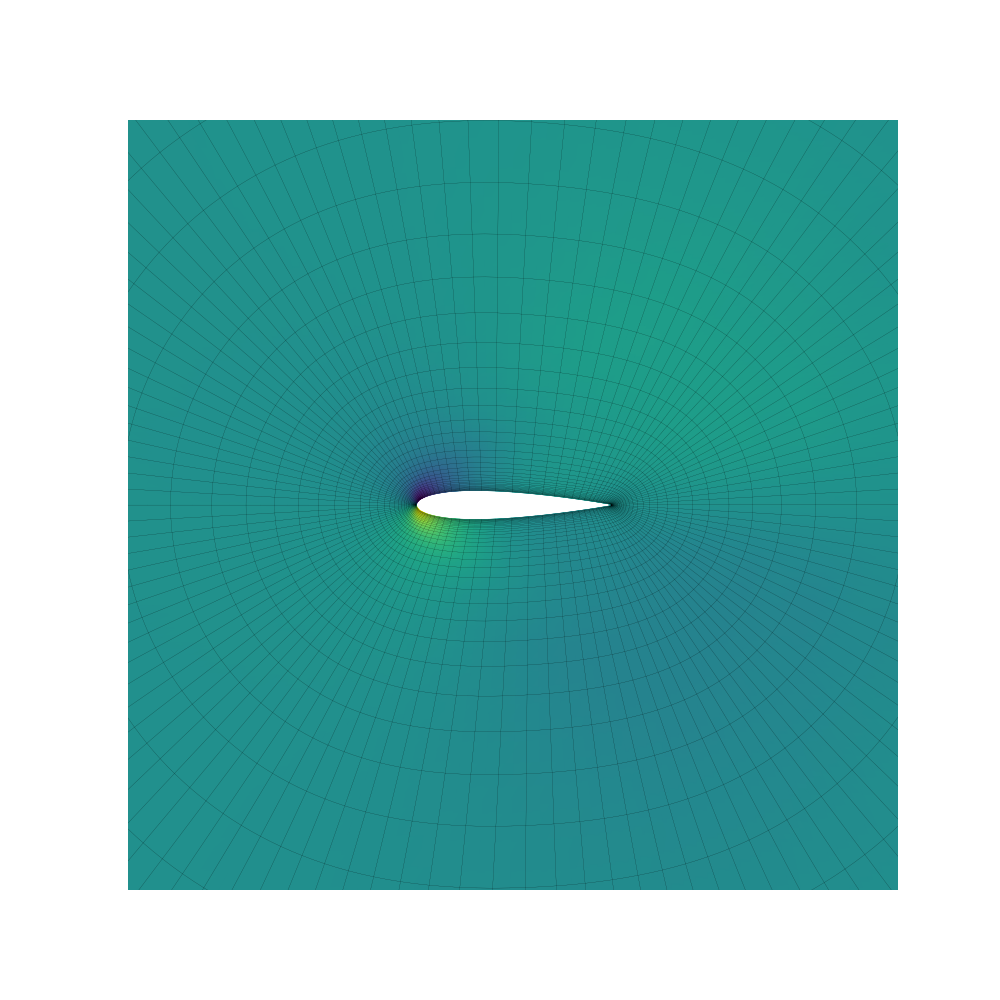
\includegraphics[trim={35mm 0 40mm 0},clip,height=0.95\textheight]{figs/bfun-p-piola-p003}
  \end{center}
\end{frame}

\end{document}
